\section{Ensuring the method is robust}
\label{sec:robustness}

The above results are quite striking; that only around 50\% of the gaseous
mass in a given halo originates from the halo's own lagrangian region calls
for a healthy dose of skepticisim. There are a number of parameters, discussed
below, where different methodologies and definitions can be applied to see
if the results are robust.

\subsection{Variations in virial radius, \rvir{}}

There is no particular, well defined, reason that the extension of the particles
in a halo to the corresponding lagrangian region should end at the virial radius
of that halo. In a similar fashion, there is not just a single definition of the
`virial radius'; in this section chagning the radius at which particles are
selected to be part of the eventual lagrangian region is explored.

The procedure for extending the lagrangian region is as follows:
\begin{enumerate}
    \item For every halo in the box, search for the centre of that halo (by
          looking for the extreme particles in each direction and finding
          their centre point, as well as taking into account the periodic
          boundaries), and the corresponding radius.
    \item Multiply this radius by a factor, such as 1.2, or 1.5
    \item For each halo in the box, use a periodic KDTree to search for the
          neighbours of the centre point within that radius, going from
          highest mass (in dark matter) to lowest mass to ensure that
          lower-mass halos `steal' from the higher mass ones, should they
          be embedded or nearby.
    \item Label these particles as belonging to the halo
    \item Re-run the original analysis with these halo definitions
\end{enumerate}

\begin{figure}
    \centering
    \includegraphics[width=\columnwidth]{generated_figures/12_rvir/component_fraction_vs_halo_mass_both.pdf}
    \caption{The analogue of Figure \ref{fig:massfrac} but after re-running
    the analysis with halos re-defined such that $r_{\rm vir, new} = 1.2
    r_{\rm vir, old}$. Note how similar the trends are. This figure has
    more noise in the errors, this is due to a smoother transition
    between halos due to the cruder methodology not fully capturing
    subhalos.}
    \label{fig:comparevirialradii}
\end{figure}
In Figure \ref{fig:comparevirialradii}, the mass fraction mass functions are
shown.There has been significant transfer between the fraction of mass in the
resulting halo from the corresponding lagrangian region to that from other
lagrangian regions. This occurs as halos that are close to each other, such as
those that are about to merge, `steal' mass from each other. The key result
from this analysis is that the fraction of mass accreted from outside of the
lagragnian region for a given halo remains relatively unchanged. This shows
that the transfer from `outside' does not primarily come from the surface of
the lagrangian region, or from gas that is mixed that lives just ouside of the
halo at $z=0$. Performing the analysis again with the halo radius scaled to
$1.5 r_{\rm vir}$ gives similar results, with more mass being transferred
between lagrangian regions and the contribution from outside any lagrangian
region remaining the same.

\subsection{The definition of lagrangian region}

\begin{figure}
    \centering
    \includegraphics[width=\columnwidth]{generated_figures/filled_regions/component_fraction_vs_halo_mass_both.pdf}
    \caption{The analogue of Figure \ref{fig:massfractions}, but with lagrangian
	regions filled out with a local nearest neighbour search of the
	nearest 64 particles, see text for details.}
    \label{fig:filledlrmass}
\end{figure}

In the above analysis, we considered a very diffuse notion of a lagrangian
region, defined particle-by-particle. Whilst increasing the virial radius
will go some way to filling the `holes' in these regions (see Figure
\ref{fig:holes}), due to the large transfer of dark matter that still occurs
(\S \ref{sec:haloindepdendent}), perhaps a different methodology is required.

Some of the holes that are present in lagrangian regions are vitally important;
these holes will collapse down to independent halos. An effort must be made to
ensure that those holes remain, whilst others are erased, with lower-mass halos
taking priority over their higher-mass cousins. With this hole-filling
exercise, it is important to note that even dark matter particles may now have
a different halo ID to lagrangain ID. The methodology that is proposed here is
as follows:
\begin{enumerate}
    \item Initially define lagrangian regions in the same way as before for
          the dark matter
    \item Find the first $n$ neighbours of every dark matter particle which
          has a lagrangian region ID of -1, i.e. it is outside of any region
    \item Overwrite the lagrangian ID of these particles with the lowest (i.e.
          corresponding to the lowest mass halo) in the group
    \item Extend the lagrangian region definition to the gas particles in
          the same way as previously, by finding the closest gas neighbour
	  particle to every dark matter particle.
\end{enumerate}
This aims to both fill out the lagrangian regions, increasing their volume-
filling fraction, ensure that no particles are `stolen' from higher-mass
halos, and reduce surface effects leading to spurious lagrangian transfer
from outside any region. See Figure \ref{fig:filledlrmass} for the results
for $n=64$ neighbours.

The majority of the transfer from outside of any lagrangian region has been
transformed into transfer from other lagrangian regions; this is because the
low-mass halos that end up being stripped of their baryons by high-mass halos
have absorbed the majority of these particles. Note how the fraction of mass
from the own lagrangian region of the halo has not changed; this means that the
surface effects on these high-mass halos are negligable.
